\section{Auswertung}
Die zu Beginn gemessene Leerlaufspannung $U_{0}$ der Monozelle und der
Innenwiderstand $R_{V}$ des Voltmeters lauten:
\begin{align*}
  U_{0} &= \SI{1,53}{\volt} \\
  R_{V} &\approx \SI{10}{\Mohm}.
\end{align*}
\noindent Um den Innenwiderstand $R_{i}$ und die Leerlaufspannung der Monozelle zu
bestimmen, wird die Klemmspannung $U_{k}$ gegen den Belastunsstrom $I$ aufgetragen.
Dies ist in Abbildung \ref{fig:plot1} zu sehen, die Steigung $a$ der Ausgleichsgeraden
entspricht dabei dem Innenwiderstand $R_{i}$ und der y-Achsenabschnitt $b$ entspricht
der Leerlaufspannung $U_{0}$.
Die Messwerte dazu finden sich in Tallele \ref{tab:tabelle1}.
\begin{table}[H]
  \centering
  \caption{Messwerte der Wärmepumpe}
  \label{tab:tabe1}
    \begin{tabular}{S S S S S S}
    \toprule
    $ t  \: / \si{\second} $ & $ p_a \: / \si{\bar} $ & $ p_b \: / \si{\bar} $ &
    $ T_1 \: / \si{\kelvin} $ & $ T_2 \: / \si{\kelvin} $ & $ P \: / \: \si{\watt} $\\
    \midrule
    0 & 5.0 & 5.0 & 293.65 & 293.65 & 0 \\
    60 & 4.7 & 6.0 & 294.15 & 293.55 & 115 \\
    120 & 4.4 & 6.4 & 295.15 & 293.15 & 118 \\
    180 & 4.5 & 6.9 & 296.35 & 291.95 & 122 \\
    240 & 4.6 & 7.0 & 297.55 & 290.95 & 125 \\
    300 & 4.6 & 7.0 & 298.85 & 289.95 & 125 \\
    360 & 4.5 & 7.2 & 300.05 & 289.15 & 123 \\
    420 & 4.4 & 7.4 & 301.15 & 288.45 & 123 \\
    480 & 4.3 & 7.8 & 302.35 & 287.65 & 122 \\
    540 & 4.2 & 8.0 & 303.55 & 286.95 & 122 \\
    600 & 4.2 & 8.1 & 304.65 & 286.25 & 121 \\
    660 & 4.1 & 8.3 & 305.75 & 285.55 & 121 \\
    720 & 4.0 & 8.5 & 306.75 & 284.95 & 121 \\
    780 & 4.0 & 8.8 & 307.75 & 284.35 & 121 \\
    840 & 3.9 & 9.0 & 308.75 & 283.75 & 121 \\
    900 & 3.8 & 9.1 & 309.65 & 283.15 & 121 \\
    960 & 3.8 & 9.2 & 310.55 & 282.55 & 122 \\
    1020 & 3.8 & 9.5 & 311.45 & 282.05 & 122 \\
    1080 & 3.7 & 9.8 & 312.25 & 281.55 & 122 \\
    1140 & 3.7 & 10.0 & 313.05 & 281.15 & 122 \\
    1200 & 3.7 & 10.0 & 313.9 & 280.65 & 122 \\
    1260 & 3.6 & 10.2 & 314.65 & 280.25 & 123 \\
    1320 & 3.6 & 10.3 & 315.35 & 279.85 & 123 \\
    1380 & 3.6 & 10.6 & 316.15 & 279.45 & 124 \\
    1440 & 3.6 & 10.8 & 316.85 & 279.15 & 124 \\
    1500 & 3.6 & 11.0 & 317.55 & 278.75 & 124 \\
    1560 & 3.6 & 11.1 & 318.25 & 278.55 & 124 \\
    1620 & 3.6 & 11.2 & 318.95 & 278.25 & 125 \\
    1680 & 3.5 & 11.4 & 319.55 & 277.95 & 125 \\
    1740 & 3.5 & 11.5 & 320.15 & 277.65 & 125 \\
    1800 & 3.5 & 11.7 & 320.75 & 277.45 & 125 \\
    1860 & 3.5 & 11.9 & 321.35 & 277.25 & 125 \\
    1920 & 3.5 & 12.0 & 321.95 & 277.05 & 125 \\
    1980 & 3.5 & 12.1 & 322.45 & 276.95 & 125 \\








      \bottomrule
    \end{tabular}
\end{table}

\begin{figure}[H]
  \centering
  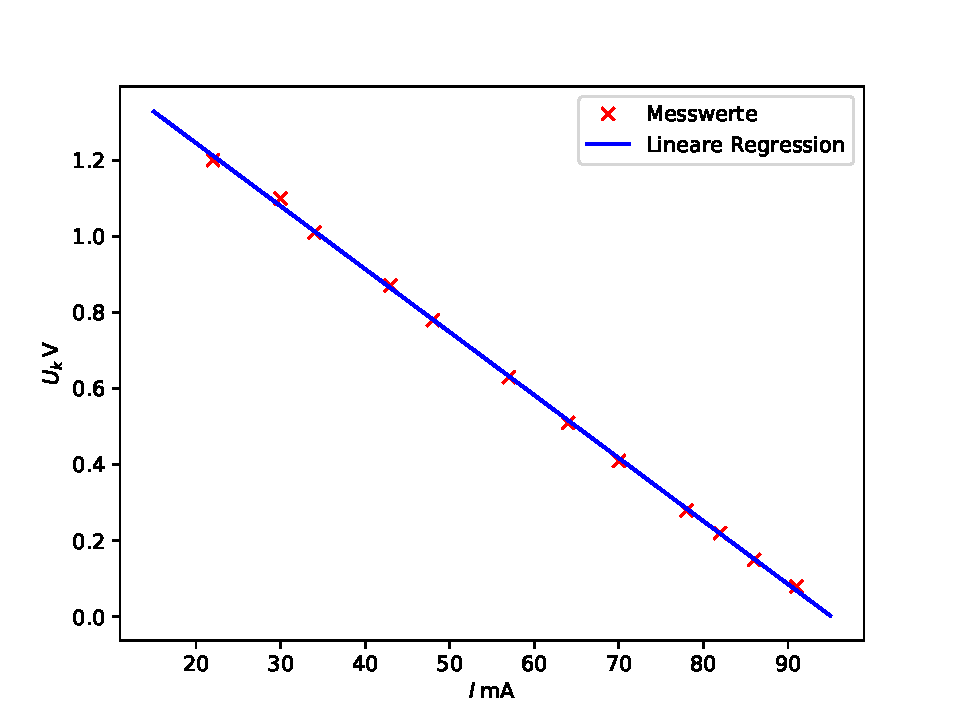
\includegraphics{plot1.pdf}
  \caption{Lineare Regression der ersten Messung: Monozelle ohne Gegenspannung.}
  \label{fig:plot1}
\end{figure}

\begin{align*}
  -a &= R_{i} = \SI{16,563(119)}{\ohm} \\
  b &= U_{0} = \SI{1,576(007)}{\volt}
\end{align*}

\noindent Die Berechnung des Innenwiderstandes $R_{i}$ und der Leerlaufspannung $U_{0}$ für
die zweite Messung, die mit einer Gegenspannung an der Monozelle durchgeführt wurde,
erfolgen äquivalent. Hier ist zu erwähnen, dass die Steigung hier im Vergleich
zu Abbildung \ref{fig:plot1} genau andersherum verläuft, da der Strom nun in entgegengesetzte
Richtung fließt. 
\begin{table}[H]
  \centering
  \caption{Wertetabelle für $\alpha$ und $C_V$.}
  \label{tab:tab2}
    \begin{tabular}{S S S S S}
    \toprule
    $ T\: \text{in}\: \si{\K} $ & $ {\alpha \cdot 10^{-6} \: \text{in}\: \si {\per\K}} $ &
    $ C_V \: \text{in}\: \si{\J\per\K\mol} $\\
    \midrule %Cv, a *10-6, Cv
    %0 & 1 & 1\\
    88.60\pm0.24 & 9.56\pm0.06 & 14.17\pm8.13  \\ %&3.6 & 318.97\pm0.85\\
    93.81\pm0.24 & 10.10\pm0.06 & 17.58\pm10.03 \\ %& 4.7 & 440.90\pm1.11\\
    99.74\pm0.24 & 10.66\pm0.05 & 15.52\pm8.84 \\ %& 5.1 & 508.68\pm1.21\\
    104.74\pm0.24 & 11.07\pm0.05 & 18.44\pm10.52 \\ %& 4.6 & 481.79\pm1.09\\
    110.94\pm0.24 &  11.54\pm0.05 & 14.86\pm8.45 \\ %& 5.3 & 587.97\pm1.27\\
    115.96\pm0.24 & 11.89\pm0.05 & 18.49\pm10.52 \\ %& 4.6 & 533.41\pm1.10\\
    121.47\pm0.24 &  12.22\pm0.05 & 16.83\pm9.57 \\ %& 4.9 & 595.21\pm1.17\\
    126.99\pm0.24 & 12.53\pm0.04 & 16.79\pm9.54 \\ %& 4.9 & 622.29\pm1.18\\
    131.58\pm0.24 & 12.77\pm0.04 & 20.42\pm11.62 \\ %& 4.2 & 552.62\pm1.01\\
    136.65\pm0.24 & 13.02\pm0.04 & 18.40\pm10.47 \\ %& 4.6 & 628.57\pm1.11\\
    141.49\pm0.24 & 13.24\pm0.04 & 19.28\pm10.97 \\ %& 4.4 & 622.54\pm1.07\\
    146.34\pm0.24 & 13.44\pm0.04 & 19.24\pm10.95 \\ %& 4.4 & 643.88\pm1.07\\
    150.95\pm0.24 & 13.62\pm0.04 & 20.22\pm11.52 \\ %& 4.3 & 649.11\pm1.05\\
    155.34\pm0.24 & 13.79\pm0.04 & 21.31\pm12.14 \\ %& 4.1 & 636.88\pm0.98\\
    159.97\pm0.24 & 13.95\pm0.04 & 20.12\pm11.47 \\ %& 4.3 & 687.89\pm1.05\\
    164.62\pm0.24 & 14.10\pm0.04 & 20.18\pm11.51 \\ %& 4.3 & 707.87\pm1.06\\
    168.79\pm0.25 & 14.23\pm0.04 & 22.54\pm12.86 \\ %& 3.9 & 658.27\pm0.95\\
    173.45\pm0.25 &  14.37\pm0.04 & 20.08\pm11.46 \\ %& 4.3 & 745.84\pm1.06\\
    178.13\pm0.25 &  14.50\pm0.04 & 20.04\pm11.44 \\ %& 4.3 & 765.94\pm1.06\\
    182.56\pm0.25 &  14.62\pm0.04 & 21.11\pm12.06\\
    192.70\pm0.25 &  14.87\pm0.04 & 18.41\pm10.47\\
    200.15\pm0.25 &  15.04\pm0.04 & 25.19\pm14.28\\
    208.87\pm0.25 &  15.23\pm0.04 & 21.43\pm12.18\\
    217.12\pm0.25 &  15.38\pm0.04 & 22.65\pm12.88\\
    225.15\pm0.25 &  15.53\pm0.03 & 23.27\pm13.24\\
    232.70\pm0.25 &  15.70\pm0.03 & 24.75\pm14.08\\
    240.53\pm0.25 &  15.74\pm0.03 & 23.84\pm13.58\\
    248.39\pm0.25 &  15.89\pm0.03 & 23.74\pm13.53& \\
    256.01\pm0.25 &  15.97\pm0.03 & 24.46\pm13.94 \\
    263.41\pm0.26 &  16.01\pm0.03 & 25.22\pm14.38 \\
    271.08\pm0.26 &  16.18\pm0.03 & 24.26\pm13.86 \\
    278.52\pm0.26 &  16.27\pm0.03 & 25.03\pm14.29&\\
    285.98\pm0.26 &  16.35\pm0.03 & 24.92\pm14.25 \\
    293.21\pm0.26 &  16.42\pm0.03 & 25.74\pm14.72 \\
    300.98\pm0.26 &  16.50\pm0.03 & 23.87\pm13.68 \\
    308.51\pm0.26 &  16.57\pm0.03 & 24.63\pm14.12\\



      \bottomrule
    \end{tabular}
\end{table}

\begin{figure}[H]
  \centering
  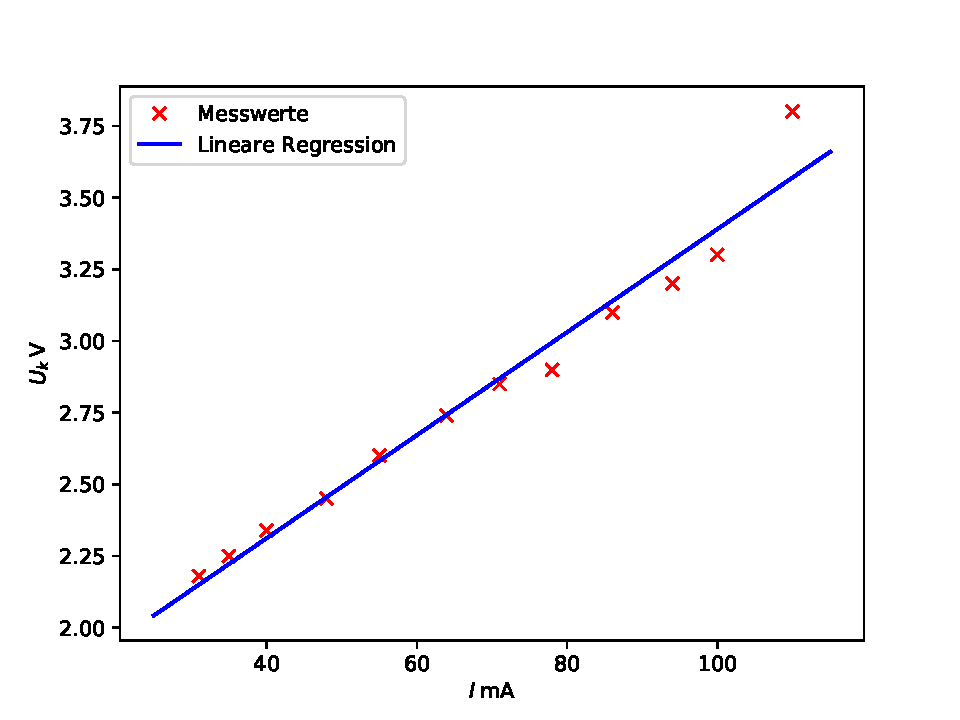
\includegraphics{plot2.pdf}
  \caption{Lineare Regression der zweiten Messung: Monozelle mit Gegenspannung.}
  \label{fig:plot2}
\end{figure}

\begin{align*}
  a &= R_{i} = \SI{17,97(102)}{\ohm} \\
  b &= U_{0} = \SI{1,593(074)}{\volt}
\end{align*}

\noindent Nun folgt die Messung einer Rechteck- und Sinusschwingung eines RC-Generators.
Die Messwerte sind in Tabelle \ref{tab:tabelle3} und dargestellt.
\begin{table}
  \centering
  \caption{Messwerte für den ersten Doppelspalt.}
   \begin{tabular}{S S| S S | S S}
    \toprule
    $x/\; \si{\mm}$& $A/\;\si{\nA}$ &
    $x/\; \si{\mm}$& $A/\;\si{\nA}$ &
    $x/\; \si{\mm}$& $A/\;\si{\nA}$ \\
    \midrule

    15.0& 4.6& 23.0& 25.0& 29.5& 6.0\\
    15.5& 4.2& 23.5& 30.0& 30.0& 5.3\\
    16.0& 4.0& 24.0& 35.0& 30.5& 4.9\\
    16.5& 4.0& 24.25& 36.0& 31.0& 4.7\\
    17.0& 4.4& 24.5& 37.0& 31.5& 4.4\\
    17.5& 5.5& 24.75& 38.0& 32.0& 4.2\\
    18.0& 6.6& 25.00& 37.0& 32.5& 3.8\\
    18.5& 7.7& 25.25& 36.0& 33.0& 3.6\\
    19.0& 8.2& 25.5& 36.0& 33.5& 3.2\\
    19.5& 8.4& 26.0& 33.0& 34.0& 3.2\\
    20.0& 8.4& 26.5& 28.5& 34.5& 3.2\\
    20.25& 8.4& 27.0& 23.0& 35.0& 3.3\\
    20.5& 8,7& 27.5& 18.0& 35.5& 3.4\\
    21.0& 9.8& 28.0& 13.5& 36.0& 3.5\\
    21.5& 12.0& 28.5& 10.0\\
    22.0& 15.0& 29.0& 7.8\\
    22.5& 20.0& 29.25& 6.7\\


   \bottomrule
  \end{tabular}
  \label{tab:tabelle3}
\end{table}

\noindent Der Innenwiderstand $R_{i}$ und die Leerlaufspannung $U_{0}$ werden erneut über Lineare Regression
bestimmt, dass ist in Abbildung \ref{fig:plot3} zu sehen.
\begin{figure}[H]
  \centering
  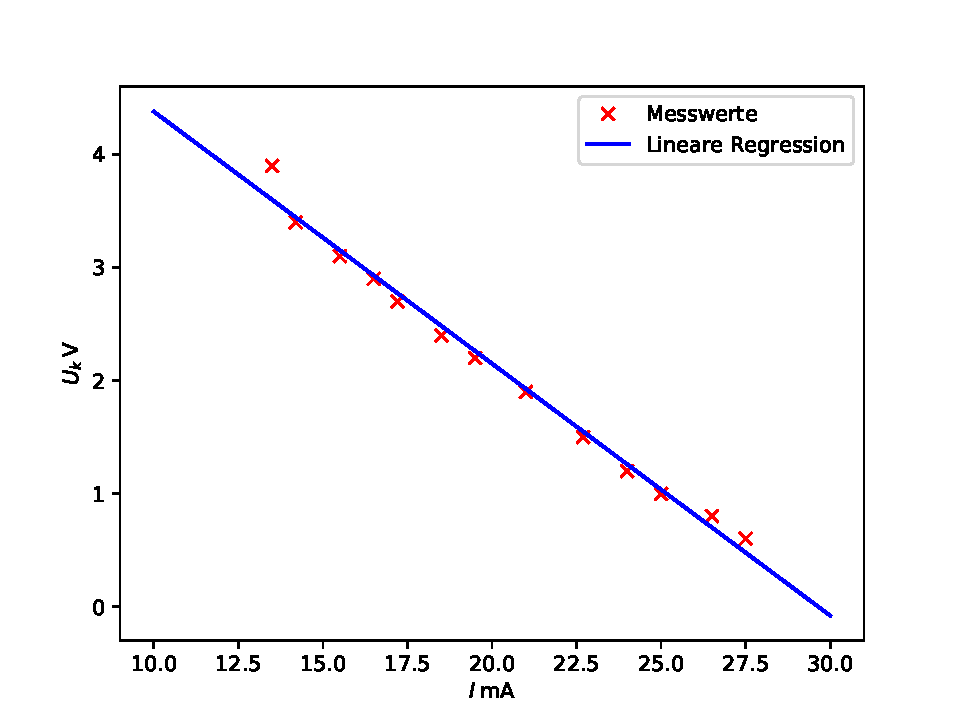
\includegraphics{plot3.pdf}
  \caption{Lineare Regression der dritten Messung: Rechteckspannung ohne Gegenspannung.}
  \label{fig:plot3}
\end{figure}
\begin{align*}
  -a &= R_{i} = \SI{222,95(703)}{\ohm} \\
  b &= U_{0} = \SI{6,610(145)}{\volt}
\end{align*}

\begin{figure}[H]
  \centering
  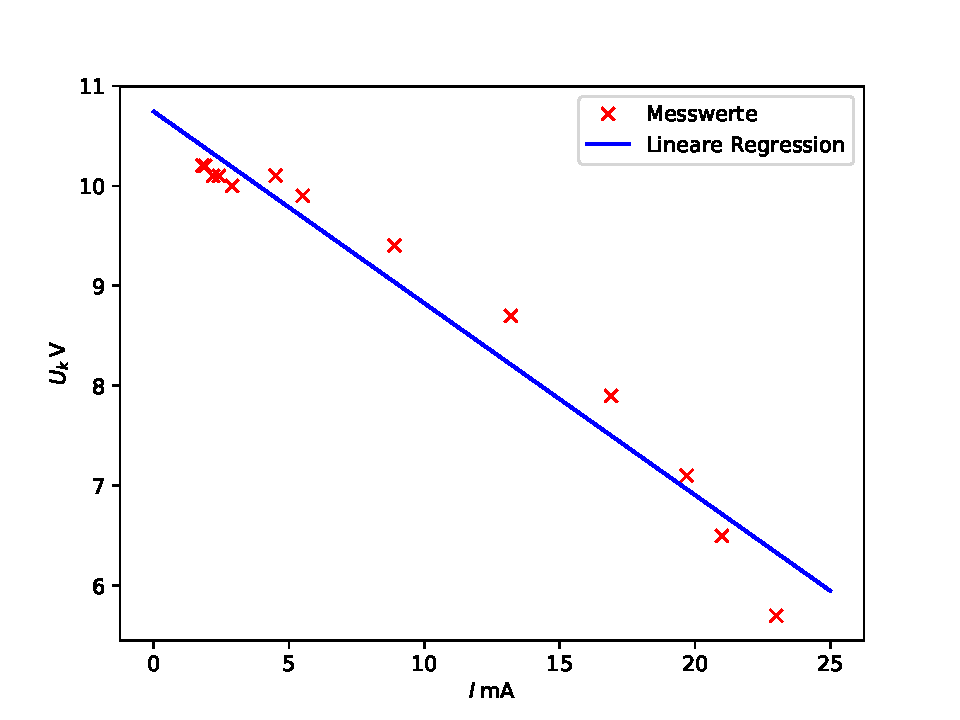
\includegraphics{plot4.pdf}
  \caption{Lineare Regression der vierten Messung: Sinusspannung ohne Gegenspannung.}
  \label{fig:plot4}
\end{figure}
\begin{align*}
  -a &= R_{i} = \SI{191,8(121)}{\ohm} \\
  b &= U_{0} = \SI{10,743(149)}{\volt}
\end{align*}

\noindent Im Folgenden wird der systematische Fehler der Leerlaufspannung $U_{0}$ berechnet,
der dadurch entsteht, dass der Widerstand der Voltmeters nicht unendlich groß sein kann.
Dafür wird die folgende Formel verwendet, die sich aus \ref{eqn:formel} ergibt, indem
die Beziehung $I=\frac{U_{k}}{R_{V}}$ verwendet wird:
\begin{equation}
  U_{0}=U_{k}+U_{k}\cdot \frac{R_{i}}{R_{a}}.
\end{equation}
Dabei entspricht $U_{k}$ dem anfangs gemessenen $U_{0}$ und $R_{a}$ ist der
Widerstand des Voltmeters. Somit berechnet sich der Fehler zu
\begin{equation}
  \Delta U_{0} = \frac{R_{i}}{R_{a}} = \SI{1.7e-9}{\ohm}.
\end{equation}
\noindent Da dieser systematische Fehler sehr klein ist, kann er vernachläsigt werden und die
Annahme eines unendlich großen Widerstandes im Voltmeter kann bestätigt werden.
Wenn das Voltmeter an dem Punkt "H", wie in Abbildung \ref{fig:schalt2}
zu sehen angeschlossen wird, entsteht ein sytematischer Fehler. Denn dann wird
das Ampermeter in der Messung mit berücksichtigt und es wird nicht die reine
Klemmspannung gemessen.

\noindent Im Folgenden werden aus den Messwerten der ersten Messreihe die
im Belastungswiderstand umgesetzte Leistung über $N=UI$ sowie der Belastungswiderstand
über $R_{a}=U_{k}/I$ berechnet, dies ist in in folgender Tabelle \ref{tab:tabelle5} zu sehen.
\begin{table}[H]
  \centering
  \caption{Bohrung 1 und 2, Vergleich der Sonden mit 1\;MHz und 2\;MHz.}
  \label{tab:tab5}
    \begin{tabular}{c c c c}
    \toprule
    Bohrung & $S_{\text{2\;MHz}}$/\;mm & $S_{\text{ 1\;MHz}}$/\;mm\\
    \midrule
    1 & 1,82 & 2,12\\
    2 & 1,83 & 1,97\\
    \bottomrule
    \end{tabular}
  \end{table}

\noindent Die hier errechneten Werte für den Belastungswiderstand werden nun gegen
die Leistung aufgetragen und mit der Theoriekurve
\begin{equation*}
  N=I²R_{a}=\frac{U_{0}^2}{(R_{a}+R_{i})^2}R_{a}
\end{equation*}
verglichen.

\begin{figure}[H]
  \centering
  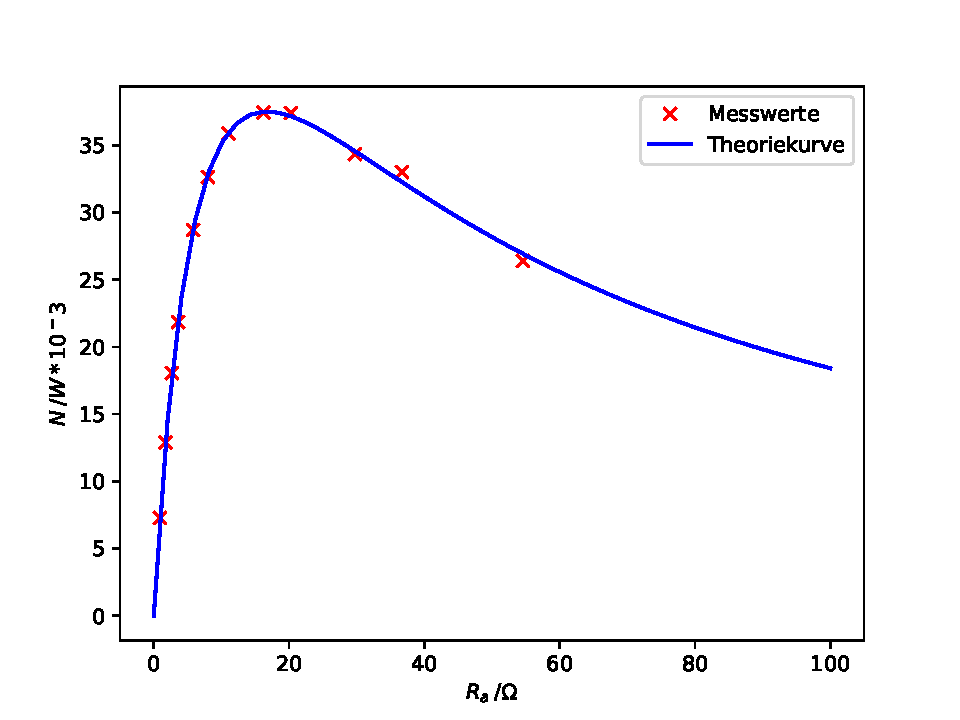
\includegraphics{plot5.pdf}
  \caption{Vergleich der Messwertw mit der Theoriekurve.}
  \label{fig:plot5}
\end{figure}
\noindent Wie in Abbildung \ref{fig:plot5} zu sehen liegen die Messwerte genau auf der
Theoriekurve. Nur zwei Messwerte weichen geringfügig von der Theoriekurve ab,
da diese Abweichung aber sehr minimal ist nicht von einem
systematischen Fehler auszugehen.

\label{sec:Auswertung}

%\begin{figure}
%  \centering
%  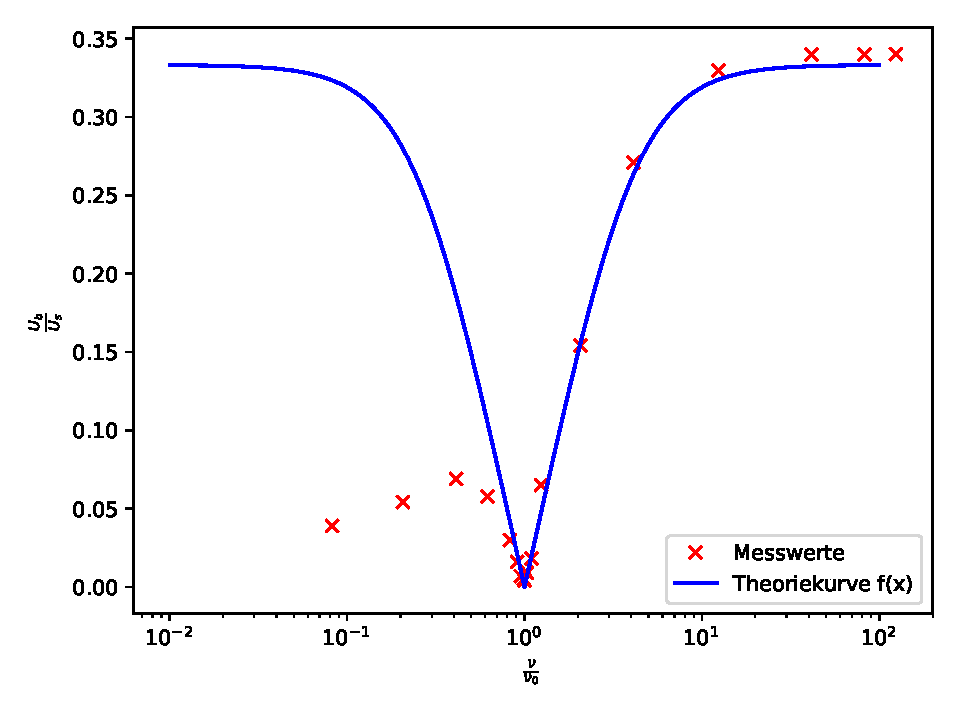
\includegraphics{plot.pdf}
%  \caption{Plot.}
%  \label{fig:plot}
%\end{figure}
